\documentclass{article}


\title{Forschungsarbeit}
\author{Laura Schillke, Sebastian Meidel, Mekong Lam }
\date{October 2018}

% Pakete laden 
\usepackage[utf8]{inputenc}
\usepackage{graphicx}
\usepackage[german]{babel}
\usepackage[default,osfigures,scale=0.95]{opensans}  %% Option 'sfdefault' only if the base font of the document is to be sans serif
\usepackage[T1]{fontenc}
% Verlinke Zitate
\usepackage{hyperref}
% Verlinke das Inhaltsverzeichnis
\hypersetup{linktocpage}
\usepackage{biblatex}
\usepackage{csquotes}
\usepackage{graphicx}
\addbibresource{mendeley_v3.bib}


%Dokument beginnt
\begin{document}

\maketitle


\newpage

\setcounter{tocdepth}{3}
\tableofcontents 



\newpage

\section{Zusammenfassung}
Bacon ipsum dolor amet shank biltong t-bone ham, ground round pastrami boudin porchetta cow fatback turkey pork tenderloin salami. Buffalo meatloaf ham hock alcatra. Boudin ground round chicken porchetta ham. T-bone spare ribs chuck fatback.

\section{Einleitung}
Bacon ipsum dolor amet shank biltong t-bone ham, ground round pastrami boudin porchetta cow fatback turkey pork tenderloin salami. Buffalo meatloaf ham hock alcatra. Boudin ground round chicken porchetta ham. T-bone spare ribs chuck fatback.

%\begin{figure}[h!]
%\centering
%
\includegraphics[scale=1.7]{universe}
%\caption{The Universe}
%\label{fig:universe}
%\end{figure}

\section{Definitionen}

\subsection{Stadt}

Haas und Neumair zufolge bezeichnet man eine Stadt als eine größere verdichtete Siedlung, die mit bestimmten Funktionen und Merkmalen charakterisiert wird \cite{HaasDefinitionWirtschaftslexikon}. Die Brockhausdefinition schreibt einer Stadt Merkmale zu wie zum Beispiel die eigene Versorgungs- und Verwaltungsstruktur, die innere Gliederung oder eine höhere Bebauungs- und Verkehrsdichte. Hinzu kommen spezielle Funktionen wie poltische Aufgaben (Haupstädte, Festungsstädte) oder wirtschaftliche Funktionen (Hansestädte, Hafenstädte, Karawanenstädte) \cite{BrockhausStadt}. Die statistischen Kriterien, die eine „Stadt“ vom „Land“ unterscheiden variieren von Land zu Land. Beispielsweise werden Städte in der Bundesrepublik Deutschland mit 
\begin{itemize}
\item 5.000 bis 20.000 Einwohnern als „Kleinstadt“,
\item 20.000 bis 50.000 Einwohnern als „Mittelstadt“,
\item ab 100.000 Einwohnern als „Großstadt“ 
\end{itemize}
bezeichnet \cite{Institutinternationaldestatistique1887BulletinStatistique}. Demgegenüber orientiert man sich in China an die Bevölkerungsdichte: 

\begin{displayquote}
In the case of cities with district establishment, the city proper refers to the whole administrative area of the district if its population density is 1 500 people per kilometre or higher [...]. \cite[S.~2]{UnitedNations2005Table2005} 
\end{displayquote}

Unabhängig von regional unterschiedlichen Kriterien lässt sich mit steigender Einwohnerzahl und -dichte einer Stadt folgern, dass auch die Anforderung an gewährleisteter Infrastruktur und Lebensmittelversorgung für die städtische Bevölkerung steigt. D.h. die Lebensmittelversorgung einer Großstadt zu gewährleisten ist schwieriger als die einer Kleinstadt. Noch größer ist die Herausforderung in Megastädten. Den Vereinten Nationen zufolge wird eine Megastadt (englisch: „Megacity“) als eine Stadt bezeichnet mit mindestens 10 Millionen Einwohnern. Im Jahr 2016 existierten 31 Megastädte und Prognosen zufolge steige die Anzahl der Megastädte im Jahr 2030 auf 41 \cite{UnitedNations2016The2016}. Tokio zählt mit 38 Millionen Einwohnern als die größte Megastadt weltweit und derzeit befinden sich die meisten Megastädte in Industrie- und Entwicklungsländern (wie in Abbildung \ref{figUrban} erkennbar). 

\begin{figure}[h]
\centering
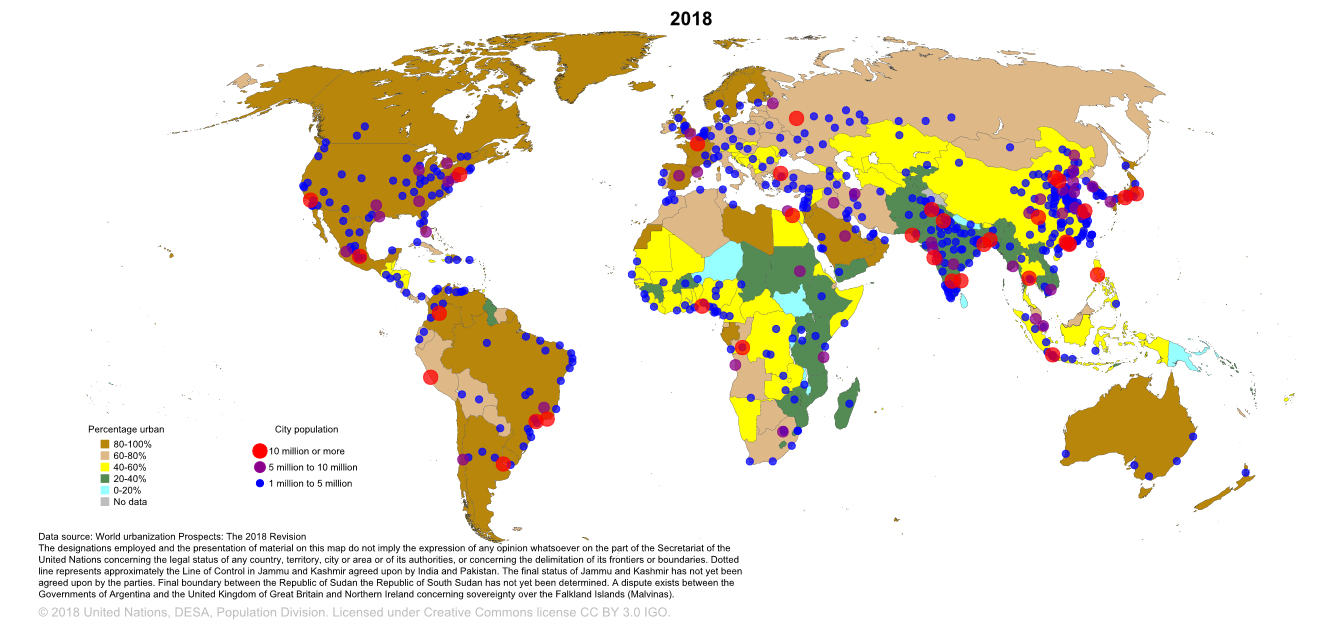
\includegraphics[width=20cm]{image_folder/CityPop_Urban.png}
\caption{Urbanisierung der Welt}
\label{figUrban}
\end{figure}

In der obigen Abbildung erkennt man, dass Nord- und Südamerika sowie Europa deutlich verstädtert sind, wohingegen viele Regionen in Afrika und Asien mehr ländliche Gebiete beinhalten. Wie gut wiederum die Lebensmittelversorgung und Infrastruktur in Megastädten ist, hängt von Megastadt zu Megastadt ab. Die Abbildung \ref{figUrbanRf} zeigt eine gute Übersicht der unterschiedlichen Verhältnisse. In dieser Forschungsarbeit der Stadtbegriff im Bezug zu ihrer fähigen Lebensmittelversorgung und Nachhaltigkeit betrachtet.


\begin{figure}[h]
\centering
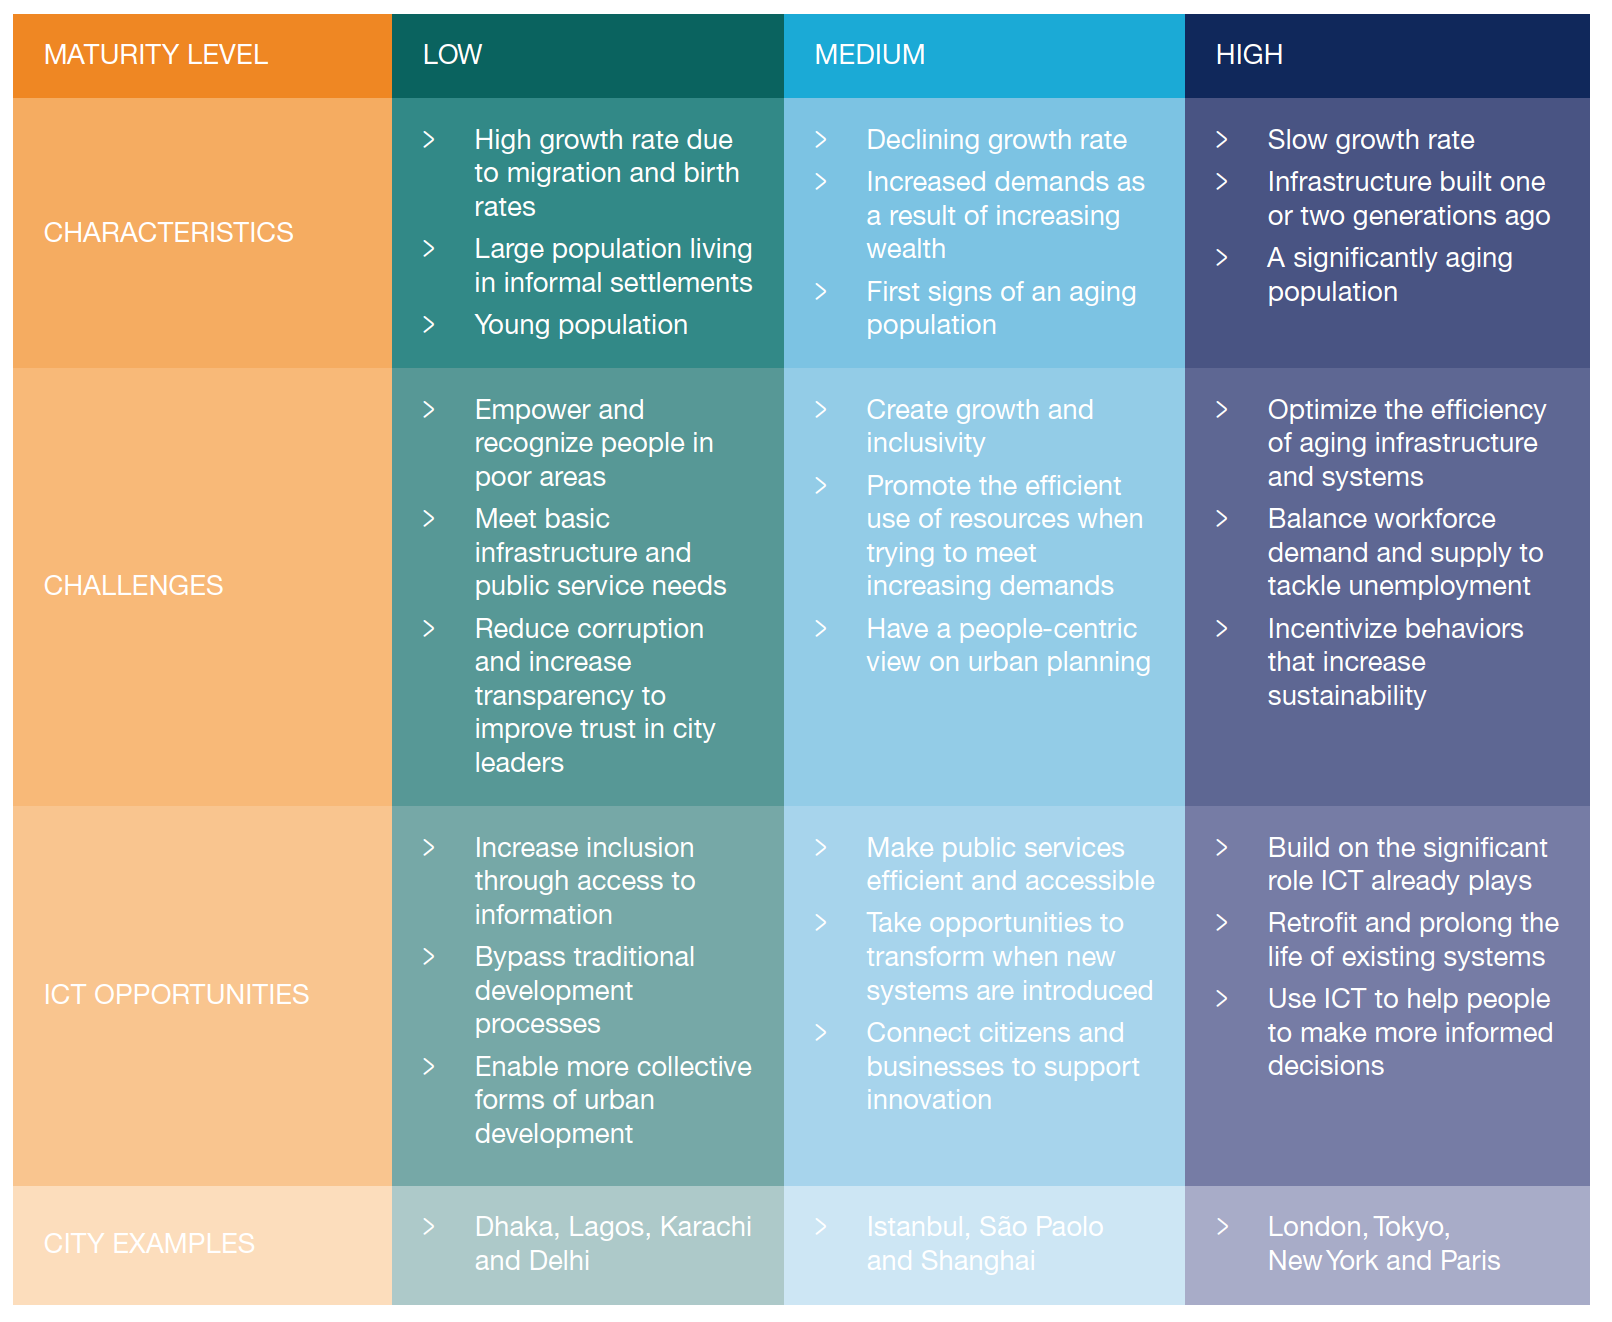
\includegraphics[width=10cm]{image_folder/urban_reifegrad.png}
\caption{Reifegrad von Megastädten}
\label{figUrbanRf}
\end{figure}

\subsubsection{Stadtökosysteme}
Stadtökosysteme sind Ökosysteme, die von Menschen erzeugt und beeinflusst werden. Wesentliche Merkmale eines Stadtökosystems sind der hohe Anteil an bebauter und versiegelter Fläche und eine hohe Bevölkerungsdichte. Genauer gesagt führt diese hohe Dichte an verschiedenen Landnutzungen dazu, dass natürlichen Ressourcen wie Wasser, Luft, Boden und Biodiversität extrem beansprucht werden. Desweiteren lässt sich über Stadtökosysteme sagen, dass ihr Erhalt von der externen Einfuhr an Lebensmitteln und Ressourcen abhängig ist  \cite[S.61]{BreusteStadtokosystemeEntwicklung}.


\subsection{Nachhaltigkeit}

Der Begriff Nachhaltigkeit ansich ist ein vielschichtiger Begriff. Er findet Verwendung in der Wirtschaft, Ökonomie, Ethik und Ökologie. So kann Nachhaltigkeit als Art und Weise des Wirtschaftens bezeichnet, „bei welcher derzeitige Bedürfnisse befriedigt werden, ohne zukünftigen Generationen die Lebensgrundlagen zu entziehen (Sustainable Development). \cite{DefinitionWirtschaftslexikonb}. Ebenso kann der Begriff als Brücke zwischen ökologischen und ökonomischen Interessen gesehen werden. Seinen Ursprung hat das Prinzip der Nachhaltigkeit in der Forstwirtschaft des 18. Jahrhunderts. Nach einer Übernutzung der Wälder und daraus resultierend knapper werdenden Holzbeständen, wurde mit Nachhaltigkeit ein Bewirtschaftungsprinzip gefordert, bei dem regenerativ gearbeitet werden sollte, das heißt “nicht mehr Holz geschlagen werden als nachwächst.“\cite{NachhaltigeBrockhaus.de}
Ab dem 19. Jahrhundert wurde zu dieser rein ressourcenökonomischen Betrachtungsweise von Nachhaltigkeit eine Umfassendere hinzugefügt, die sämtliche Funktionen des Waldes in Betracht zieht.

politische Umsetzung Nachhaltigkeit
Ergebnisse des Gipfels von Rio zur Nachhaltigkeit




Der Begriff Nachhaltigkeit kann in stark und schwach eingeteilt werden.\cite{Nachhaltigkeit}


\begin{itemize}
\item starke Nachhaltigkeit: Erhaltung der natürlichen Ressourcen steht im Vordergrund.Es beruht auf der Annahme, dass Naturgut nicht durch andere Kapitalformen ersetzt werden kann,
\item schwache Nachhaltigkeit beruht auf der Annahme das Kapital- oder Naturgut durch andere Kapitalformen erstz werden kann.
\end{itemize}
Konfliktpotenzial zwischen den Vertretern jeweiliger Positionen treten vor allem bei der Frage auf, "wie heute verursachte, aber zukünftig auftretende Umweltschäden beziehungsweise Ressourcenknappheiten zu bewerten sind.\cite{NachhaltigeBrockhaus.de}

\subsubsection{Kritik am Begriff der nachhaltigen Entwicklung}\cite{NachhaltigeBrockhaus.de}
Die übermäßige Verwendung des Begriff führt bei vielen Kritikern zu Misstrauen. Folgende Meinungen werden vertreten:

\begin{itemize}
\item Begriff sei überladen und als Sammelbegriff für alles Gute, was unerfüllbare Erwartungen wecke
\item Nachhaltige Entwicklung sei utopisch und eine Illusion
\item Beliebigkeit des Begriffs: “Unter der Flagge der nachhaltigen Entwicklung könne man trotzdem für komplett gegensätzliche Dinge eintreten.”
\item Meinung: Nachhaltigkeit sei inhaltslos und habe nur rhetorische FUnktionen, was die Leitbildfähigkeit des Begriffs außer Kraft setze
\end{itemize}

\subsubsection{Ökologische Nachhaltigkeit}
„Die ökologische Nachhaltigkeit bezieht sich allgemein auf das Überleben und den Gesundheitszustand von Ökosystemen.“ \cite{DefinitionWirtschaftslexikonc}  Sie bezeichnet einen weitsichtiger und rücksichtsvoller Umgang mit natürlichen Ressourcen. Sofern die ökologische Nachhaltigkeit vernachlässigt wird, kann dies dazu führen, dass bestimmte Ressourcen unbrauchbar oder unwiderruflich zerstört werden mit dem Ergebnis, dass auf diese Weise jegliche weitere Entwicklungen unmöglich werden. Laut Berding und Bukow in :Die kompakte Stadt der Zukunft Auf dem Weg zu einer inklusiven und nachhaltigen Stadtgesellschaft (s.95) \cite{BerdingWolf-DietrichBukowKarinCudakHrsgDieStadtgesellschaft} gewinnt das Thema Nachhaltigkeit für die Stadtentwicklung an Wichtigkeit. 

\subsubsection{Nachhaltige Entwicklung}
 Dieser Begriff wurde von N. abgeleitet. In der internationaler Politik und bei gesellschaftlichen Bewegungen wird er als Leitbild eingesetzt. Ziel der Nachhaltigen Entwicklung ist eine dauerhalfte und gerechten Bewirtschaftung der Erde. \cite{NachhaltigeBrockhaus.de} In der Agrar- und Ernährungswirtschaft zielt der Begriff auf eine " dauerhafte Nutzung von Ressourcen bei gleichbleibender bzw. wachsender Effektivität". \cite{oppenhauser2010nachhaltigkeit} Im internationalen Sprachraum hat sich der Begriff Sustainable Development als Definition dieses Leitbild gefestigt.
 
 Konkrete Umsetzungsmethoden von Nachhaltiger Entwicklung stellen in Entwicklungsländern hauptsächlich Entwicklungsaspekte in den Vordergrund, in den industrialisierten Ländern geht es um den langfristigen Schutz und Erhalt der natürlichen Lebensgrundlage. 

\subsubsection{Konfliktpotenziale bei der Umsetzung von Nachhaltiger Entwicklung}

Die gerechte verteilung der endlichen ressorcen (global commons)

Das Rio-Abkommen aus dem Jahr 1992 wurde neben der Frage nach der Verantwortung für die Verursachung von Umweltproblemen die “Gerechtigkeitsfrage […] von zahlreichen Kommentatoren so beantwortet, dass im Prinzip jeder Mensch weltweit das gleiche Recht hat, die globalen Gemeinschaftsgüter in nachhaltiger Weise zu nutzen. Dieser Interpretation wird entgegengehalten, dass sie regional unterschiedliche Bedürftigkeiten und kulturelle Besonderheiten ignoriere.” cite{NachhaltigeBrockhaus.de}Ebenso besteht der "Einwand, dass neben den unterschiedlichen Bedürftigkeiten auch das unterschiedliche Leistungsvermögen berücksichtigt werden müsse. Demnach sei das zulässige Nutzungsniveau eines Staates nicht nach der Größe seiner Bevölkerung, sondern nach seinem Beitrag zur globalen Wertschöpfung zu bestimmen." \cite{NachhaltigeBrockhaus.de}

\begin{figure}[htp]
\centering
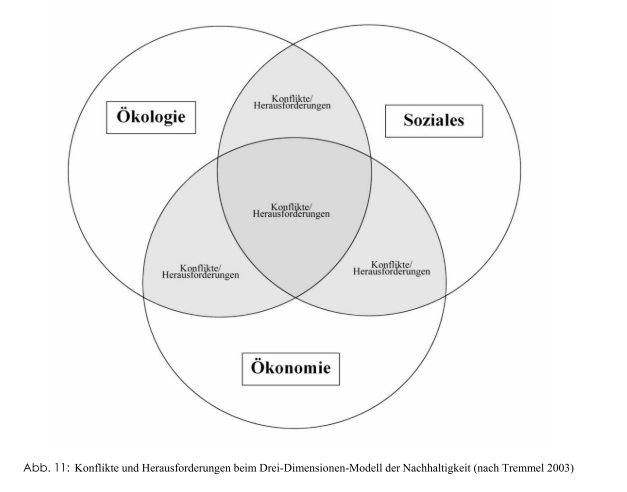
\includegraphics[width=10cm]{image_folder/dreidimensionenmodell_der_N.png}
\caption{3-dim-Modell}
\label{fig:3-dimensionen Modell}
\end{figure}

Konfliktpoltenzial besteht ebenfalls bei der Priorisierung von Lösungsvorschlägen. Eine Nachhaltige Lösung im sozialen Sinn kann auf Kosten von ökologischer Nachhaltigkeit gehen und umgekehrt. Genauso kann auch eine Win-Win Situation entstehen.

Länder des Südens stellen bislang die sozialen und ökonomischen Aspekte in den Vordergrund, Länder des Nordens wird dadurch die Hauptlast bei der Lösung der bestehenden Probleme im Ökologischen Bereich zugeschrieben. Die Länder des Nordens stellen ök. Apekt in den Vordergrund, nicht zuletzt weil sie es sich leisten können. SIe fordern gleichzeitig Lösungsinitative von Ländern des Südens

\begin{figure}[htp]
\centering
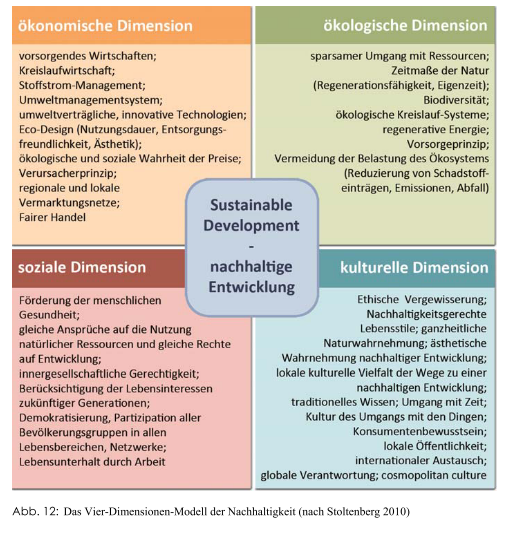
\includegraphics[width=10cm]{image_folder/vierdimensionenmodell_der_N.png}
\caption{4-dim-Modell}
\label{fig:4-dimensionen Modell}
\end{figure}

\subsubsection{Ökoeffizienz}
 Der World Business Council of Sustainable Development (WBCSD) hat " für Ökoeffizienz die folgenden Kriterien erstellt: die Bereitstellung wettbewerbsfähiger Produkte, die menschliche Bedürfnisse befriedigen, die Lebensqualität fördern und dabei die Umweltauswirkungen und Ressourcenintensität während des gesamten Produktlebens minimieren." \cite{OkoeffizienzBrockhaus.de}

Als Ökoeffizient werden Strategien und Konzepte bezeichnet, die sich dazu eignen nachhaltige Produktionsmethoden umzusetzen. Die Kriterien sind laut des World Business Council of Sustainable Development (WBCSD) – ein Zusammenschluss international tätiger Unternehmen, der das Ziel hat, Wirtschaftswachstum und Nachhaltigkeit in Einklang zu bringen  Folgende:
\begin{itemize}
\item geringer Einsatz natürlciher Ressourcen
\itemg eringe Umweltbelastung
\item zu ersteren beiden im Vergleich hoher Ertrag
\end{itemize}

Ökoeffizienz kann u. a. erreicht werden durch:
\begin{itemize}
\item Minimierung des Material- und Energieverbrauchs pro Produktmenge,
\item Verwendung recyclingfähiger Materialien,
\item Einsatz erneuerbarer Ressourcen, Vermeidung des Einsatzes toxischer Substanzen,
\item Erhöhung der Lebensdauer beziehungsweise des Nutzens eines Produktes.
\end{itemize}
Methodische Ansätze zur Messung der Ökoeffizienz von Produkten sind:
\begin{itemize}
\item Stoffstrommanagement,
\item die Umweltbilanz
\item Ökoeffizienz-Analyse Bewertungsmethode der BASF." Sie entstand 1995 und bewertet die Wirtschaftlichkeit eines Produkts im Verhältnis zu der Umweltbelastung, die sie ausübt. Betrachtet wird der gesamte Lebensweg des Produkts beginnend bei der Rohstoffgewinnung über die Herstellung und Verwendung bis zur Entsorgung.
\end{itemize}https://www.brockhaus.de/ecs/enzy/article/ökoeffizienz (Quelle des gesamten Abschnitts)

ökologischer Fußabdruck
"Die (Natur-)Fläche, die zur Aufrechterhaltung der Energie- und Materialflüsse einer Wirtschaftsein-heit wie z. B. einer Stadt benötigt wird, ist deren ökologischer Fußabdruck. Er ist ein Werkzeug zur Bilanzierung des menschlichen Naturverbrauchs und wird in globalen Hektaren angegeben (vgl. Wackernagel & Rees 1997, 23–25). „Der ökologische Fußabdruck misst so die‚ ökologische Tragfä-higkeit’ einer Bevölkerung“ (Wackernagel & Rees 1997: 25)."(Zitaat ausGrundlagen einer nachhaltigen Entwicklung S.5)

\begin{figure}[htp]
\centering
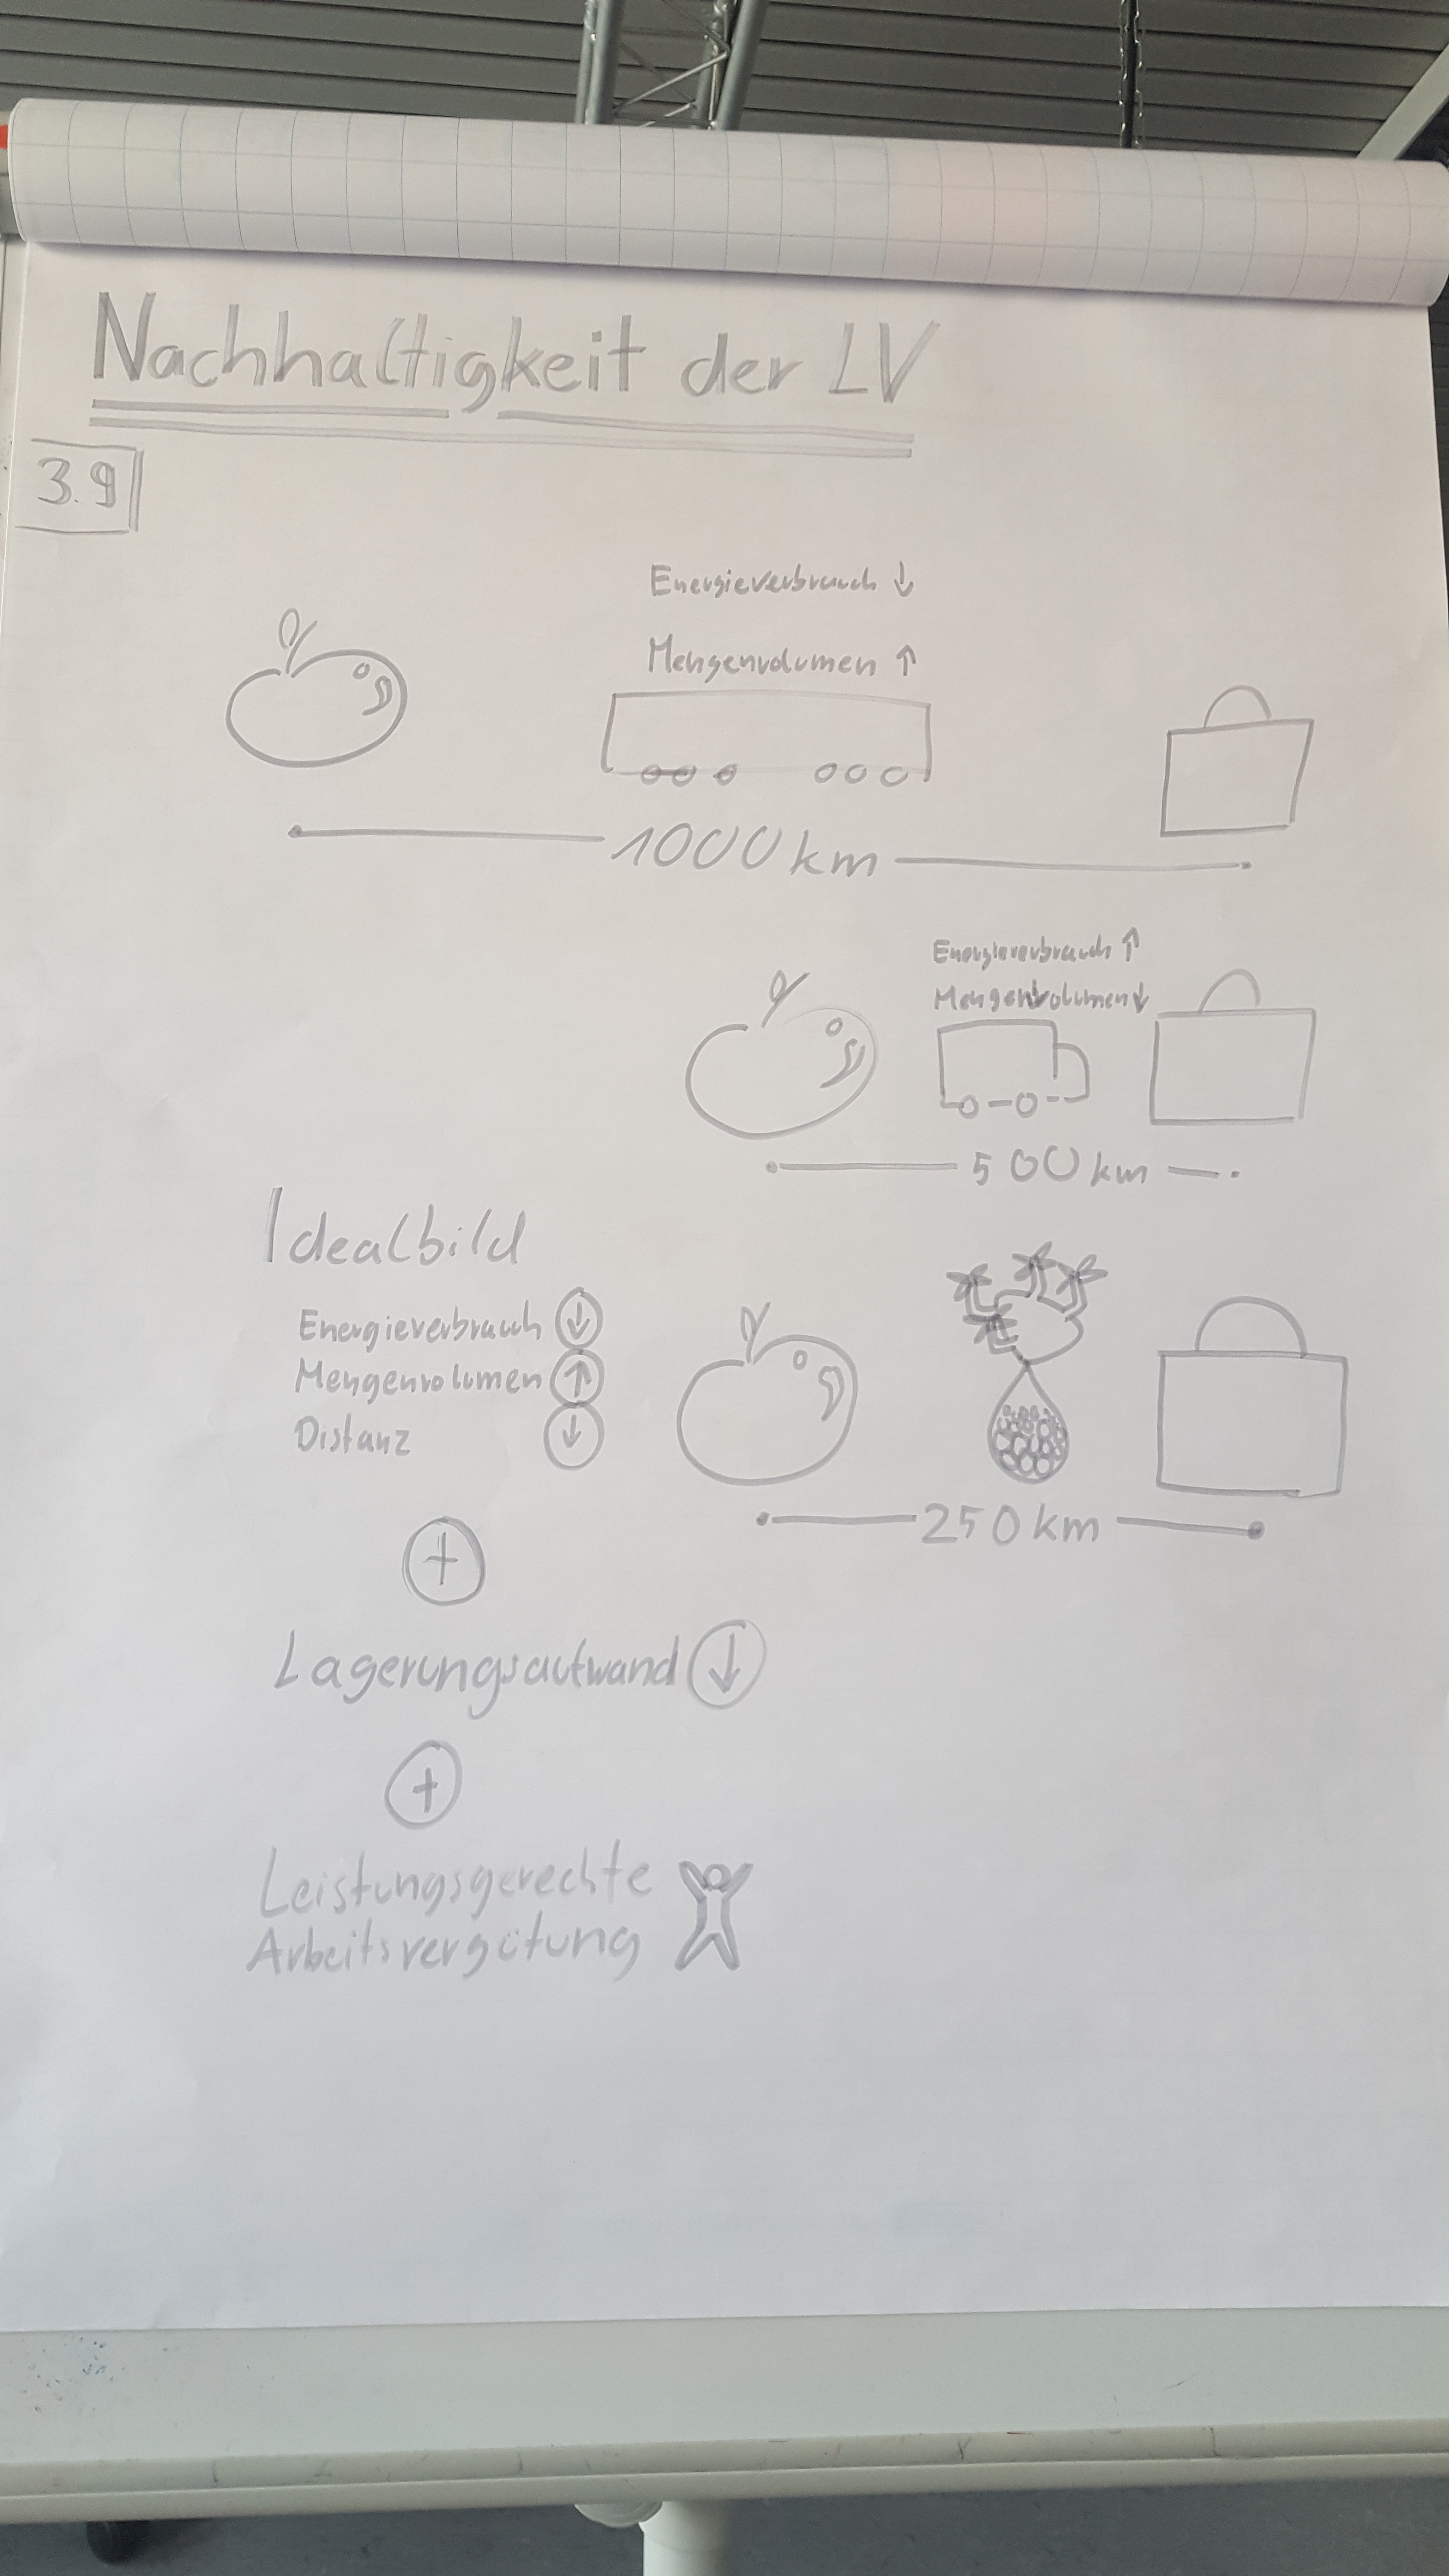
\includegraphics[width=5cm]{image_folder/skizze1.jpg}
\caption{Nachhaltigkeit der LV}
\label{fig:Skizze_Nachhaltigkeit}
\end{figure}

\subsection{Geschichte der Urbanisierung}

Betrachtet man die Entwicklung und bisherige Ausgestaltung von Städten, kann man leicht ein bestimmtes System dahinter entdecken.
Neben der eher durchdachten Verortung der Städte fand eine klare Differenzierung zum ländlichen Raum statt. Städte oder Siedlungen wurden
zwar seit je her in Gebieten gegründet die Versorgung durch Trinkwasser und Nahrung sicherstellen, dennoch wurden Nahrungsmittel häufig
aus dem Umland in die Städte befördert. Hierbei stellt die Megametropole New York ein klares Beispiel dar. Die Entwicklung der Stadt zeigt
durch ihre verdichtete urbane Struktur eindeutig eine Entwicklung, die die rurale Landwirtschaft oder ländliche Flächen "aussperrt". Dennoch
ist die Stadt durch die Nähe zum Fluss und der ausgebauten Infrastruktur für eine Versorgung für Nahrungsmittel aus der ruralen Landwirtschaft
gut gerüstet. Die Stadt selbst fungiert hierbei lediglich als Lebensraum und infrastrukturelle Anlaufstelle.
Die ländliche Abwesenheit war also ein Selbstverständnis für viele frühe Städte.

Dabei existieren bereits seit mehr als 100 Jahren Stadtpläne durch ambitionierte Stadtplaner die das rurale Land als solches für das Leben in einer
Stadt als essentiellen Bestandteil ansehen. Betrachtet man zum Beispiel einmal die Vision des britischen Sadtplaners Ebenezer Howard. Seine Vision der
Gartenstadt bildet noch heute ein Vorbild für moderne Stadtplaner. In seinem Buch "Garden Cities of Tomorrow" welches bereits 1898 verfasst wurde vertritt er das Konzept eines raffinierten Zusammenspiels von ruraler Landwirtschaft und urbanen Gebieten. Er betont zudem dass es sich bei den
Gärten nicht nur um angelegte Ziergärten und Erholungsorte sowie Freizeitparks handelt sondern auch um "Freiräume", die Platz für den Anbau von
Nutzpflanzen und der Aufzucht von Nutztieren bietet. Dieser Punkt wurde in den kommenden Jahren durch nachfolgende Stadtplaner oft übergangen. Für den nachfolgenden Stadtbau verkam der Aspekt der UL zur Gestaltung von mühevoll angelegten vermeintlich natürlichen Ziergärten, die Grünflächen und
Erholungsgebiete in die Städte bringen sollten. Neben den frühen Gedanken an eine Landwirtschaft innerhalb städtischer Strukturen ist der Aspekt der
Versorgung und Infrastruktur ebenfalls betrachtet worden.

\begin{figure}[htp]
\centering
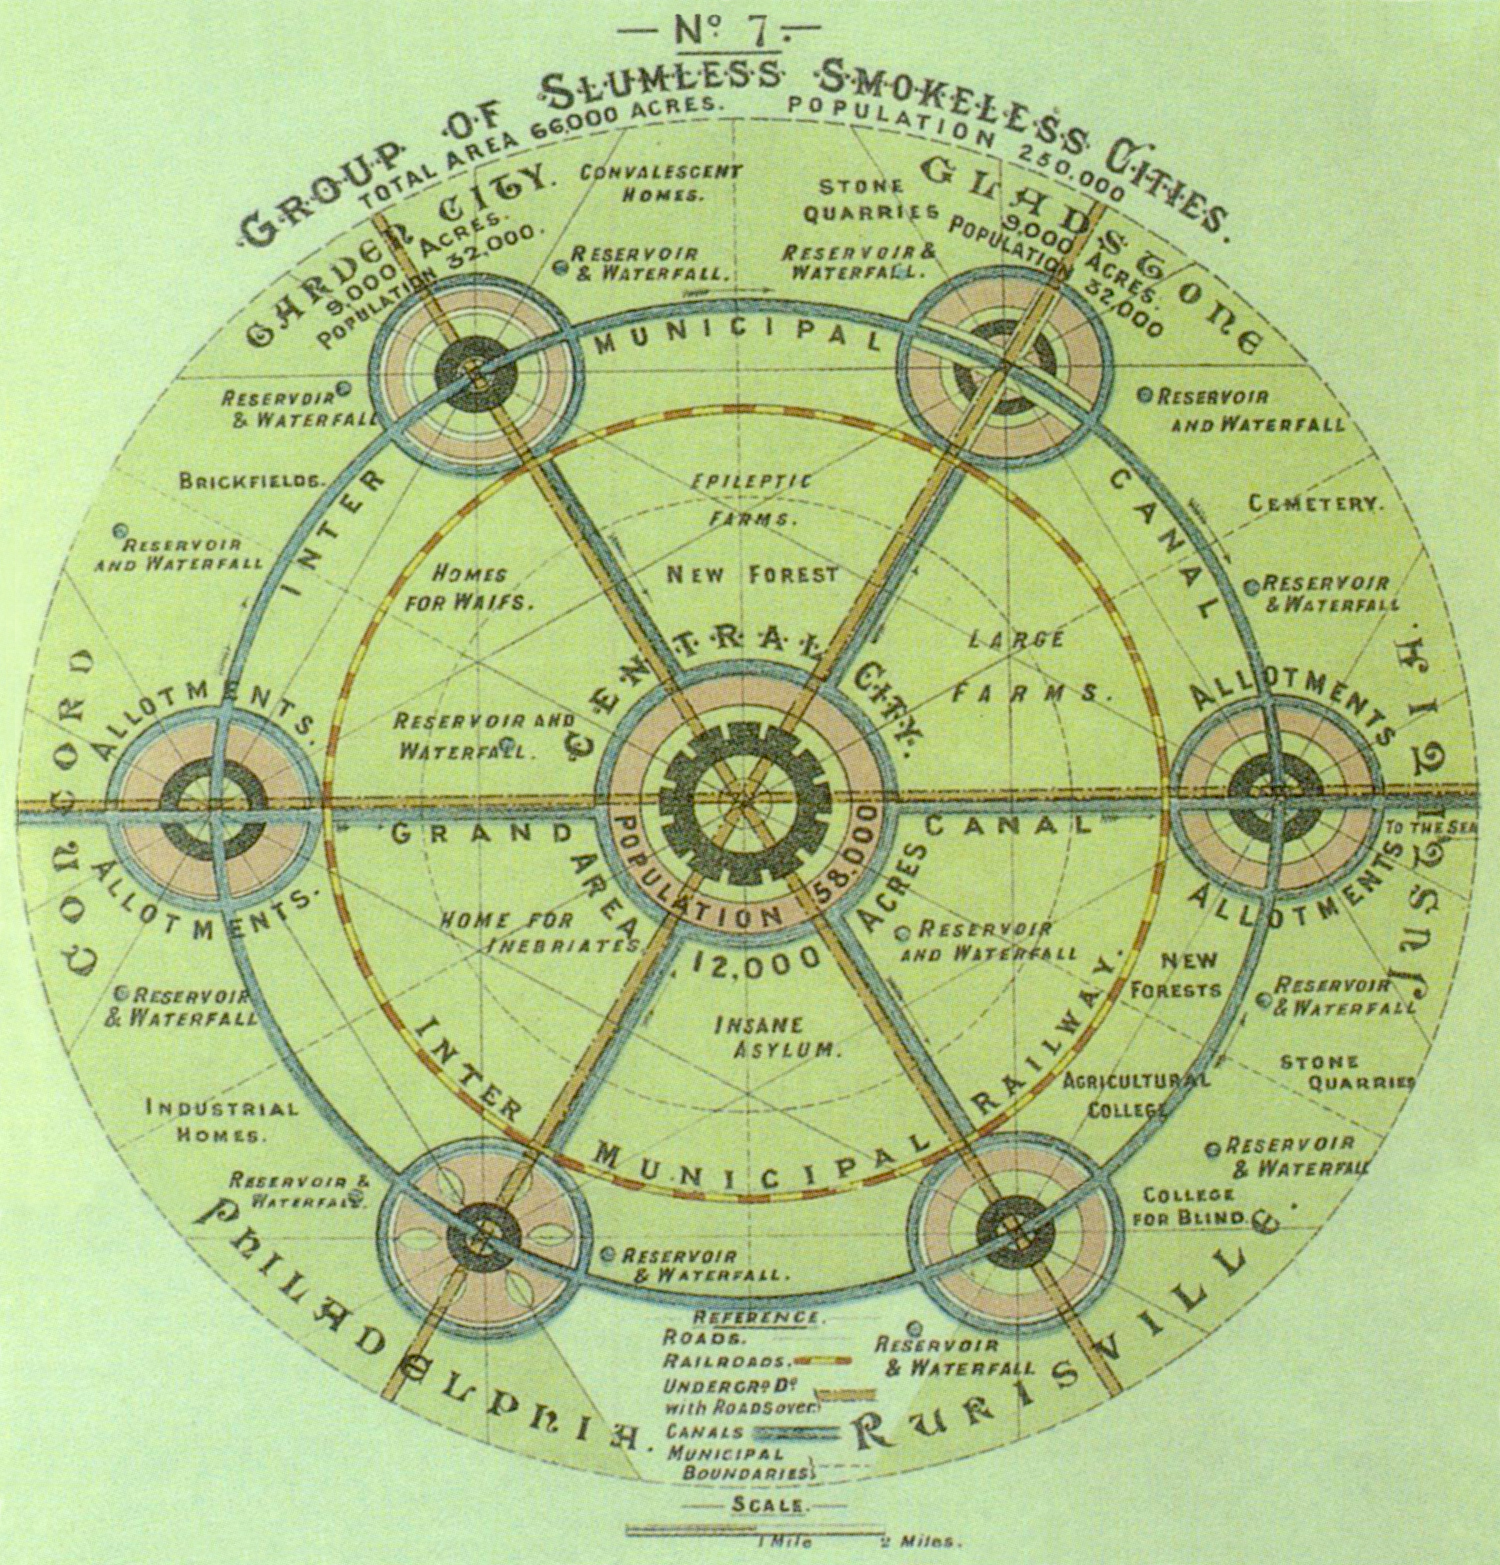
\includegraphics[width=10cm]{image_folder/GardenCityConcept_EbenezerHoward.jpg}.jpg}
\caption{Konzept der Gartenstadt von Ebenezer Howard}
\label{fig:GardenCityConcept_EbenezerHoward}
\end{figure}



\newpage
\listoffigures
\printbibliography
\end{document}
